\documentclass[border=4pt]{standalone}
\usepackage{amssymb}
\usepackage{tikz}
\usetikzlibrary{calc,shapes.misc}

\begin{document}
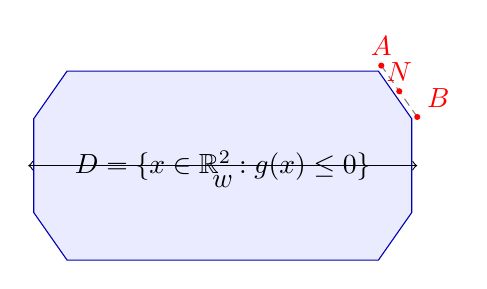
\begin{tikzpicture}
  \node[shape=chamfered rectangle,draw=blue!70!black,fill=blue!8,
    chamfered rectangle angle=35,chamfered rectangle xsep=5mm,
    chamfered rectangle ysep=3mm,minimum width=48mm,minimum height=24mm,
    outer sep=2pt] (D) at (0,0) {$D=\{x\in\mathbb R^2:g(x)\leq0\}$};

  \draw[densely dashed,gray] (D.before north east) -- (D.north east) -- (D.after north east);
  \fill[red] (D.before north east) circle (1.1pt) node[above right] {$B$};
  \fill[red] (D.north east) circle (1.1pt) node[above] {$N$};
  \fill[red] (D.after north east) circle (1.1pt) node[above] {$A$};
  \draw[<->] (D.west) -- node[below] {$w$} (D.east);
\end{tikzpicture}
\end{document}
